% !TeX root = RJwrapper.tex
\title{\texttt{quickmapr}: Simplified mapping and basic interactivity.}
\author{by Jeffrey W. Hollister}

\maketitle

\abstract{%
There are many packages that already exist or are in active development
that support the visualization of spatial data in R. However, there
seems to be a gap for those that need to quickly view, compare, and
interactively explore the results of a given spatial analysis without
first having to convert to a different coordinate reference system.
Functionality for the current release (v0.2.0) simplifies mapping of
multiple \texttt{sf}, \texttt{sp} or \texttt{raster} layers, and also
provides interactive zooming, panning, labelling, selecting, and
identifying. These tools are intended for use within an active spatial
analysis workflow and not for production quality maps. Additionally,
\texttt{quickmapr} does not make any assumptions about coordinate
reference systems and leaves managing of projections to the analyst.
This paper introduces the package and shows examples of its typical use.
}

\subsection{Introduction}\label{introduction}

Spatial data analysis capabilities in R have been steadily growing over
the last several years. We are now to the point where nearly all
Geographic Information Systems (GIS) functionality can be accomplished
without leaving R. The one area that had lagged behind was spatial data
visualization and interactivity. This too is changing rapidly.
Initially, spatial data visualization had been handled via base plotting
methods (e.g from \CRANpkg{sp} or \CRANpkg{raster}) or via additional
plotting packages such as
\CRANpkg{ggplot2}\citep{pebesma2005classes, bivand2013asdar, raster, ggplot2}.
While these methods provide the ability to make high quality maps, they
do not provide interactivity, a hallmark of GIS.

To address this, most solutions (e.g. \CRANpkg{ggmap},
\CRANpkg{leaflet}, \CRANpkg{mapview} etc.) have relied on javascript
libraries or other web APIs \citep{ggmap, leaflet, mapview}. These
provide a modern interface, with a rich set of basemaps, but all assume
a geographic coordinate system or Web Mercator coordinate reference
system. In the case of typical spatial data analysis workflow it is
often desirable to quickly map the resultant spatial datasets in the
projection chosen for the analysis. Currently, this is not possible with
the most used javascript libraries.

I developed \CRANpkg{quickmapr} to fill this gap and provide spatial
data analysts with a tool to quickly map multiple layers and interact
with the resultant map without having to utilize various APIs or
external libraries and without having to re-project data. The goals of
this paper are to describe the basic usage of \pkg{quickmapr}, show
several examples of its use, and outline changes expected in future
versions. We also briefly discuss the contribtuion that \pkg{quickmapr}
makes to the existing suite of spatial data visualization tools in R.

\subsection{Basic usage}\label{basic-usage}

The basic workflow for using \pkg{quickmapr} is as follows:

\begin{enumerate}
\def\labelenumi{\arabic{enumi}.}
\tightlist
\item
  Use the \code{qmap()} function to create a \code{qmap} object. This
  object holds the data and pertinent information about the current
  visualization environment (e.g.~symbology, zoom/pan extent, etc.).
  This first step is acheived with:
\end{enumerate}

\begin{Schunk}
\begin{Sinput}
library(quickmapr)
data(lake)

qm <- qmap(elev,lake,samples,buffer)
\end{Sinput}

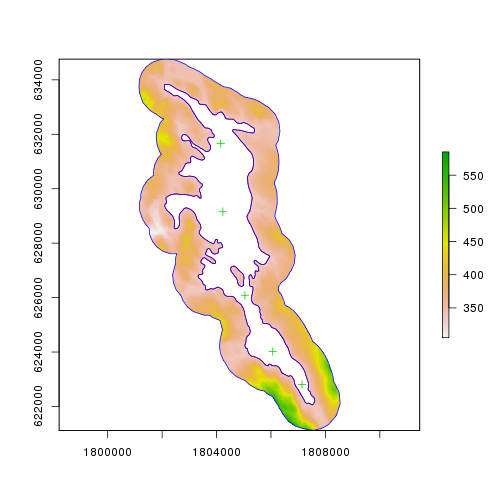
\includegraphics{hollister_files/figure-latex/workflow-1} \end{Schunk}

\begin{enumerate}
\def\labelenumi{\arabic{enumi}.}
\setcounter{enumi}{1}
\tightlist
\item
  With a \code{qmap} object created you may interact with the map using
  the various \pkg{quickmapr} functions.
\end{enumerate}

\subsection{\texorpdfstring{The \code{qmap} function and
object}{The  function and object}}\label{the-function-and-object}

The \code{qmap} object is an S3 object, with a class of ``qmap'' and
contains a list with 11 items. These items are:

\begin{itemize}
\tightlist
\item
  map\_data: a list of all data used to create the map.
\item
  map\_extent: the current map extent. Initially it is the maximum
  extent that encompasses all of \texttt{map\_data}, but changes to
  reflect the currently selected zoom extent.
\item
  orig\_extent: original extent of the map. Does not change and is used
  to reset map.
\item
  draw\_order: controls draw order of \texttt{map\_data}. Defaults to
  order of \texttt{map\_data}
\item
  colors: outline, line, or point colors for vector datasets in
  \texttt{map\_data}
\item
  fill: fill colors for polygons
\item
  map:
\item
  basemap: A character string indicating which type of basemap to fetch
  from the \href{}{USGS National Map}
\item
  col\_tbl:
\item
  values:
\item
  resolution: Resolution of \texttt{basemap}. Controls quality of image
  with smaller resolution resulting in higher quality image, but slower
  drawing.
\end{itemize}

Currently, the only implemented default method is for plotting which may
be accessed either through \texttt{qm}, \texttt{plot(qm)} or
\texttt{print(qm)}.

\subsection{Zooming and panning}\label{zooming-and-panning}

\subsection{Identification and
selection}\label{identification-and-selection}

\subsection{Basemaps from the USGS National
Map}\label{basemaps-from-the-usgs-national-map}

\subsection{Summary}\label{summary}

This file is only a basic article template. For full details of
\emph{The R Journal} style and information on how to prepare your
article for submission, see the
\href{https://journal.r-project.org/share/author-guide.pdf}{Instructions
for Authors}.

\bibliography{hollister}

\address{%
Jeffrey W. Hollister\\
U.S. Environmental Protection Agency\\
Office of Research and Development\\ National Health and Environmental Effects Research Laboratory\\ Atlantic Ecology Division\\ 27 Tarzwell Drive\\ Narragansett, RI 02882\\
}
\href{mailto:hollister.jeff@epa.gov}{\nolinkurl{hollister.jeff@epa.gov}}

